\documentclass[10pt]{report}
\usepackage[margin=0.9in]{geometry}
\usepackage{fontspec}
\usepackage[explicit]{titlesec}
\usepackage{setspace}
\usepackage{enumitem}
\usepackage{changepage}
\usepackage{paracol}
\usepackage{url}
\usepackage{polyglossia}
\usepackage{hyperref}
\usepackage{graphicx}
\usepackage{subcaption}


% polyglossia
\setmainlanguage{portuges}

% fontspec
\setmainfont{FreeSerif}
\setsansfont{FreeSans}
\setmonofont{FreeMono}

% titlesec
\titleformat{\chapter}[display]{\onehalfspacing\bfseries\centering}{\Large \chaptertitlename~\thechapter}{1.5em}{\Large\MakeUppercase{#1}}
\titleformat{\section}[display]{\bfseries\normalsize\centering}{\thesection\ \ \ \ \MakeUppercase{#1}}{-1em}{}
\titleformat{\subsection}[display]{\bfseries\normalsize\centering}{\thesubsection\ \ \ \ #1}{-1em}{}
\titleformat{\paragraph}[runin]{\scshape\bfseries}{}{1em}{#1}

\newenvironment{circumstances}{
    \titleformat{\subsection}[display]{\normalsize}{\thesubsection\ \ \ \ \MakeUppercase{##1}}{-1em}{}
    \titleformat{\paragraph}[runin]{\scshape}{}{1em}{}

    \begin{paracol}{2}
        \setlength{\columnseprule}{0.4pt}
        \setlength{\columnsep}{2em}
} {
    \end{paracol}
}

% table of contents
\setcounter{tocdepth}{3}
\setcounter{secnumdepth}{6}
\setcounter{chapter}{0}

\begin{document}

\title{Euroscope Manual}
\author{Portugal vACC}

\maketitle

\tableofcontents

\chapter*{Prefácio}

\paragraph*{} Este documento pretende explicar alguns detalhes em relação ao pacote de LPPC,
nomeadamente, os ficheiros de vistas radar, as TAGs, e as novidades na área \textit{Display
Settings}.

\paragraph*{} Antes de mais, o pacote está criado de forma a ser bastante simples abri-lo. Bastará
arrastar, toda, a pasta para a pasta \path{%userprofile%\Documents\Euroscope}. Depois será
unicamente necessário abrir o Euroscope como sempre, tendo em atenção que se utiliza o novo
\path{LPPC_CTR.prf}.

\paragraph*{} De notar que na primeira vez será necessário configurar o seguinte:
\begin{itemize}
    \item Posição de controlo (escolher no menu drop-down) e servidor;
    \item Nome, senha e rating do CTA;
    \item Microfone, auscultador e botão PTT (Push-To-Talk).
\end{itemize}

\chapter{Definições}

\textit{Nota. — Em adição ao disposto neste capítulo, considere as definições em ICAO Doc. 4444,
Chapter 1 Definitions.}

\paragraph*{} Quandos os seguintes termos ou acrónimos são usados neste documento têm o seguinte
significado:

\paragraph*{\textit{RIV.}}
\label{def:riv}
\hangindent=\parindent
Região de Informação de Voo.

\paragraph*{\textit{CTA.}}
\label{def:cta}
\hangindent=\parindent
TODO

\paragraph*{\textit{TAG(s).}}
\label{def:tags}
\hangindent=\parindent
Etiqueta associada a um determinado avião visível no radar.
\paragraph*{} \textit{Nota. — Ver capítulo \hyperref[cap:tags]{TAGs} para uma descrição detalhada das várias
TAGs disponíveis.}

\paragraph*{\textit{COPX.}}
\label{def:copx}
\hangindent=\parindent
Ponto de coordenação, \textit{coordination point}, é utilizado para
referência ao ponto para o qual a aeronava foi ou será instruída para seguir para.

\paragraph*{\textit{TSSR.}}
\label{def:tssr}
\hangindent=\parindent
Codigo transponder.

\chapter{Vistas radar}
\label{cap:vistas}

\paragraph*{} Vistas radar são definidas em ficheiros \path{.asr} e definem, entre outros, o centro
de radar, zoom, TAGs activas, e \textit{display settings}. Pode encontrar as várias configurações
disponíveis em \path{%userprofile%\Documents\Euroscope\LPPC\ASR}.

\paragraph*{} No propósito deste documento, vistas radar são caracterizadas pela posição que as
controla. Por exemplo a vista \path{LPPC_CTR} aplica-se à posição de Lisboa Control, e começará com
uma vista a abranger todo o espaço aéreo da RIV de Lisboa. Por outro lado, \path{LPPT_GND}
aplica-se, por defeito, ao aeroporto de Lisboa.

\paragraph*{} Estão disponíveis, por ordem alfabética, as seguintes vistas:
\begin{itemize}
    \item \path{LPFR_APP}
    \item \path{LPFR_GND}
    \item \path{LPFR_TWR}
    \item \path{LPMA_APP}
    \item \path{LPMA_GND}
    \item \path{LPMA_TWR}
    \item \path{LPPC_CTR}
    \item \path{LPPR_APP}
    \item \path{LPPR_GND}
    \item \path{LPPR_TWR}
    \item \path{LPPT_APP}
    \item \path{LPPT_GND}
    \item \path{LPPT_TWR}
\end{itemize}

Por pré-definição estão visíveis 9 padrões de espera (ADSAD, EKMAR, RINOR, UMUPI em LPPT;
GIMAL em LPFR; DIVUT, RETMO em LPPR; ABUSU, FUSUL em LPMA).

Por pré-definição estão ligados os sectores LPPC East e LPPC West.

\section{Navegação entre vistas}

\paragraph*{} Para selecionar uma determinada vista, em \texttt{OPEN SCT - Open} selecione o ficheiro
\texttt{asr} correspondente. Alternativamente é possível definir teclas de atalho para vistas
específicas em \texttt{OTHER SET - General Settings - Page 2}.

\paragraph*{} Para navegar entre vistas utilize a tecla \texttt{F7}. Para repor a condição da vista
actual, por exemplo após mover o radar para focar um determinado avião de interesse, utilize a
combinação de teclas \texttt{CTRL + HOME}.

\chapter{TAGs}
\label{cap:tags}

\paragraph*{} Apesar de existerem diversas configurações e formatos atribuídos a tags para
representar informações diferentes sobre aeronaves, neste capítulo pertende-se abordar as de maior
interesse às posições assumidas pelo controlador.

\paragraph*{} As informações presentes em uma tag serão enumeradas da esquerda para a direita e de
cima para baixo. Separadas em 3 classificações de formatos que mencionadas elas têm o seguinte
significado:

\paragraph*{\textit{Correlacionada.}}
\hangindent=\parindent
O formato de tag atribuída a uma aeronave com a qual o controlador ainda não interagiu.

\paragraph*{\textit{Expandida.}}
\hangindent=\parindent Não sendo necessárimente, pode considerar a tag atribuída a uma aeronave
quando assumida pelo controlador.

\paragraph*{\textit{Detalhada.}}
\hangindent=\parindent
A tag expandida quando sobreposta pelo cursor.

\paragraph*{}
\textit{Nota 1. — Todas as tags assumem que a aeronave está correlacionada com um plano de voo.}

\paragraph*{}
\textit{Nota 2. — As tags disponibilizadas intendem ser um ponto de partida para o controlador
ajustar a sua preferência, se assim o desejar, os sendo o mais próximo das utilizadas pelo ACC
de Lisboa a data que foi possível apurar.}

\begin{figure}[h]
    \centering
    \begin{subfigure}[b]{0.3\textwidth}
        \begin{center}
            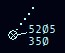
\includegraphics[width=0.37\textwidth]{figures/correlated-tag}
            \caption{Uma tag correlacionada}
            \label{fig:correlated}
        \end{center}
    \end{subfigure}
    ~ %add desired spacing between images, e. g. ~, \quad, \qquad, \hfill etc.
      %(or a blank line to force the subfigure onto a new line)
    \begin{subfigure}[b]{0.3\textwidth}
        \begin{center}
            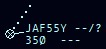
\includegraphics[width=0.6\textwidth]{figures/expanded-tag}
            \caption{Uma tag expandida}
            \label{fig:expanded}
        \end{center}
    \end{subfigure}
    ~ %add desired spacing between images, e. g. ~, \quad, \qquad, \hfill etc.
    %(or a blank line to force the subfigure onto a new line)
    \begin{subfigure}[b]{0.3\textwidth}
        \begin{center}
            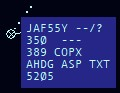
\includegraphics[width=0.66\textwidth]{figures/detailed-tag}
            \caption{Uma tag detalhada}
            \label{fig:detailed}
        \end{center}
    \end{subfigure}
    \caption{Exemplos de tags}\label{fig:tag-examples}
\end{figure}

\section{Informação das TAGs}

\paragraph*{Correlaciona} Em todas as famílias esta indica o código \textit{TSSR}, e altitude
reportada pela aeronave. Sendo que não serve para propósito de assumir controlo da aeronave, é
pretendido apenas dar indicação de posição espacial da aeronave.

\subsection{PT vACC – NORM}
\label{sec:tag-norm}

\paragraph*{} Para utilização nas posições de Torre e Aproximação, garante que o controlador tem as
informações necessárias para o correcto sequenciamento e espaçamento em fase final de aproximação.

\paragraph*{Expandida} Indicativo de chamada, próximo controlador, altitude, altitude
temporária (atribuída pelo CTA), e velocidade (\textit{ground speed}).

\paragraph*{Detalhada} É adicionado o COPX para coordenar directos, a informação de rumo e
velocidade instruída pelo CTA, caixa de texto livre, e o código transponder.

\paragraph*{} Todos campos que identificam uma instrução dada ao piloto são possíveis de serem
alterados directamente na tag clicando sobre os mesmos para revelar interface apropriada, por
exemplo, clicando sobre a velocidade deverá revelar uma lista de velocidades em espaços
apropriados.

\subsection{PT vACC – RDUC}
\label{sec:tag-rduc}

\paragraph*{} Recomendada para as posições de centro.

\paragraph*{Expandida e Detalhada} Semelhante a \hyperref[sec:tag-norm]{PT vACC – NORM} apenas não é mostrada
informação de velocidade.

\subsection{PT vACC – GND RDR}

\paragraph*{} Recomendada para as posições de chão.

\paragraph*{Expandida} Indicativo de chamada.

\paragraph*{Detalhada} Indicativo de chamada e código de identificação do tipo de aeronave.

\subsection{PT vACC – XPDR}

\paragraph*{Expandida} Ver \hyperref[sec:tag-norm]{PT vACC – NORM}.

\paragraph*{Detalhada} Semelhante a \hyperref[sec:tag-rduc]{PT vACC – RDUC} tem ainda informação do
código TSSR.

\paragraph*{} \textit{Nota. — Não é utilizada por nenhuma posição, deverá ser utilizada por decisão do CTA.}

\chapter{Display Settings}

\paragraph*{} Este capítulo aborda as diferentes características do espaço aéreo disponíveis para
serem adicionadas ao radar. As secções mencionadas referem-se aos vários nós na árvore do
\textit{Display settings dialog} do Euroscope, em \texttt{OTHER SET – Display Settings}.

\paragraph*{} \textit{Nota 1. — Este capítulo aborda as várias informações disponíveis de ter
visíveis no radar, não sendo necessáriamente as que estarão activas. Para um detalhe das
informações activas por defeito ver capítulo \hyperref[cap:vistas]{Vistas Radar}.}

\paragraph*{} \textit{Nota 2. — Algumas das secções disponíveis são propositádamente ignoradas
neste capítulo, apenas secções de especial interesse serão abordadas.}

\section{Stars}

\paragraph*{} Para além de poder activar o desenho das diferentes STARs para os vários aerportos,
esta secção incluí ainda os padrões de espera.

\section{ARTCC boundary}

\paragraph*{} Incluí todos os limites laterais da RIV de Lisboa, sectores, e áreas restritas. Todos
os sectores estão conforme designado pela NAV Portugal, prefazendo um total de 6 sectores
diferentes, \textit{NORTH}, \textit{CENTER}, \textit{SOUTH}, \textit{DEMOS}, \textit{VERAM}, e
\textit{MADEIRA}. Com excepção dos três últimos referidos, todos os sectores se subdividem em
\textit{lower} (até FL245) e \textit{upper} (desde FL245).

\paragraph*{} Para facilatar as várias posições que podem assumir os vários sectores, estão ainda
disponíveis os pseudo setores \textit{LPPC East} (\textit{DEMOS}, \textit{VERAM}, e
\textit{MADEIRA}) e \textit{LPPC West} (\textit{NORTH}, \textit{CENTER}, e \textit{SOUTH}).

\paragraph*{} \textit{Nota. — Limites laterais dos lower e upper sectores, diferem apenas na
fronteira com Espanha, onde os sectores lower seguem a fronteira terrestre os sectores upper
extendem até aos pontos de coordenação com Espanha.}

\section{ARTCC low boundary}

\paragraph*{} Esta secção incluí as várias caracteristicas de interesse circundantes dos aeroportos
sob controlo de trafego aéreo. TMA, MRVA, \textit{Tower} CTR, e rotas especiais VFR.

\section{Free Text}

\paragraph*{} Todos as caracteristicas do espaço referidas anteriormente podem ter o código de
identificação das mesmas visíveis no radar bastante activar o correspondente nesta secção.

\paragraph*{} A secção \textit{SCT2} incluí os códigos das aéras restritas.

\paragraph*{} \textit{Nota. — A secção DynPoints deverá ser ignorada e mantida desactivada, serve
apenas de suporte a outras caracteristicas do radar.}

\end{document}
